\begin{figure*}[tb]
\centering
\definecolor{resultNavy}{HTML}{24557A}
\definecolor{resultTeal}{HTML}{2A7F78}
\definecolor{resultGray}{HTML}{7B8791}
\begin{minipage}[t]{0.485\textwidth}
\centering
{\small\textbf{(a)} Retrieval ordering at a fixed pool}\par\vspace{1.5mm}
\begin{tikzpicture}[x=1cm,y=1cm,font=\footnotesize]
  \draw[black!35,line width=0.45pt] (2.55,0.50) -- (6.15,0.50);
  \foreach \x/\lab in {2.55/0.20,3.75/0.24,4.95/0.28,6.15/0.32} {
    \draw[black!35,line width=0.45pt] (\x,0.44) -- (\x,0.56);
    \node[anchor=north,text=black!65] at (\x,0.39) {\lab};
  }
  \node[anchor=east,align=right] at (2.36,2.30) {Pool $R@1000$};
  \node[anchor=east,align=right] at (2.36,1.15) {Submitted $R@k_q$};

  \draw[-{Stealth[length=2.2mm]},line width=0.85pt,resultNavy!75]
    (5.361,2.30) -- (6.027,2.30);
  \fill[resultGray] (5.361,2.30) circle (2.1pt);
  \fill[resultNavy] (6.027,2.30) circle (2.7pt);
  \node[anchor=north,text=resultGray] at (5.361,2.17) {0.2937};
  \node[anchor=south,text=resultNavy] at (6.027,2.43) {0.3159};

  \draw[-{Stealth[length=2.2mm]},line width=0.85pt,resultNavy!75]
    (3.162,1.15) -- (3.579,1.15);
  \fill[resultGray] (3.162,1.15) circle (2.1pt);
  \fill[resultNavy] (3.579,1.15) circle (2.7pt);
  \node[anchor=north,text=resultGray] at (3.162,1.02) {0.2204};
  \node[anchor=south,text=resultNavy] at (3.579,1.28) {0.2343};
\end{tikzpicture}
\end{minipage}\hfill
\begin{minipage}[t]{0.485\textwidth}
\centering
{\small\textbf{(b)} RAG coverage--support trade-off}\par\vspace{1.5mm}
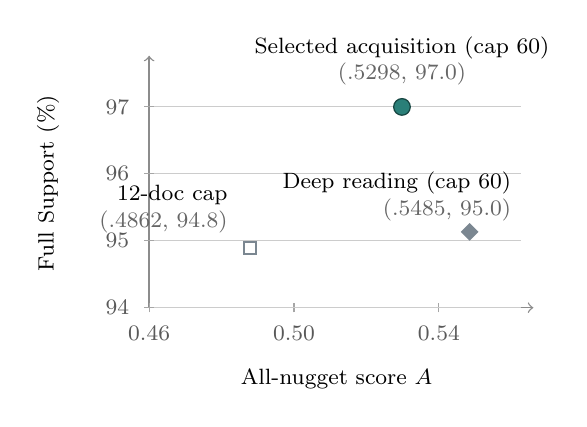
\begin{tikzpicture}[x=1cm,y=1cm,font=\footnotesize]
  \draw[->,black!45,line width=0.5pt] (1.40,0.72) -- (6.28,0.72);
  \draw[->,black!45,line width=0.5pt] (1.40,0.72) -- (1.40,3.92);
  \foreach \x/\lab in {1.40/0.46,3.24/0.50,5.08/0.54} {
    \draw[black!35] (\x,0.66) -- (\x,0.78);
    \node[anchor=north,text=black!65] at (\x,0.61) {\lab};
  }
  \foreach \y/\lab in {0.72/94,1.57/95,2.42/96,3.27/97} {
    \draw[black!20] (1.46,\y) -- (6.12,\y);
    \draw[black!35] (1.34,\y) -- (1.46,\y);
    \node[anchor=east,text=black!65] at (1.27,\y) {\lab};
  }
  \node[anchor=north] at (3.78,0.06) {All-nugget score $A$};
  \node[rotate=90,anchor=south] at (0.38,2.30) {Full Support (\%)};

  \draw[resultGray,line width=0.8pt] (2.605,1.40) rectangle +(4.4pt,4.4pt);
  \node[anchor=south east,align=right] at (2.52,1.55)
    {12-doc cap\\\textcolor{black!60}{(.4862, 94.8)}};

  \fill[resultGray] (5.471,1.57) -- +(3.2pt,3.2pt) -- +(0pt,6.4pt)
    -- +(-3.2pt,3.2pt) -- cycle;
  \node[anchor=south east,align=right] at (6.12,1.70)
    {Deep reading (cap 60)\\\textcolor{black!60}{(.5485, 95.0)}};

  \fill[resultTeal] (4.611,3.27) circle (3.0pt);
  \draw[resultTeal!55!black,line width=0.45pt] (4.611,3.27) circle (3.0pt);
  \node[anchor=south,align=center] at (4.611,3.42)
    {Selected acquisition (cap 60)\\\textcolor{black!60}{(.5298, 97.0)}};
\end{tikzpicture}
\end{minipage}
\caption{Development-set comparison of the selected systems and their
nearest development alternatives. Panel (a) reports the observed change from
pre-deep-tail to deep-tail ordering on the same 5,000-document Retrieval
pool. Panel (b)
plots RAG all-nugget coverage against Full Support; it illustrates the
observed coverage--citation-support trade-off. Exact values and metric definitions appear
in Tables~\ref{tab:retrieval-cutoff} and~\ref{tab:rag-results}.}
\label{fig:development-summary}
\end{figure*}
